\documentclass[aspectratio=169,10pt]{beamer}
\usetheme{metropolis}
\usepackage{booktabs}
\usepackage{graphicx}
\usepackage{xcolor}
\graphicspath{{../../figures/shapes/}}

\definecolor{vizblue}{HTML}{2A78D6}
\definecolor{vizorange}{HTML}{EB6834}
\setbeamercolor{progress bar}{fg=vizblue}
\setbeamercolor{title separator}{fg=vizblue}
\setbeamercolor{alerted text}{fg=vizorange}
\metroset{numbering=fraction, progressbar=frametitle}

\title{RTF alert-compression}
\author{Mat Madhavacheril, Nayan Patel}
\date{October 2026}

\begin{document}

\maketitle

% ---------------------------------------------------------------------------
\begin{frame}{Question and setup}
  \textbf{Does the \texttt{LightCurveCompressor} latent carry image information at all?}
  Test it with no photometry, metadata or GP features.
  \vspace{0.3em}
  \begin{columns}[T]
    \column{0.55\textwidth}
    \footnotesize
    \begin{itemize}
      \item One identical all-zero photometry token per source, so the transformer
        CLS output is a constant (verified):
        $z = \mathrm{bottleneck}(\mathrm{const} + \mathrm{ImageTower}(\text{stamp}))$.
      \item Stamps: $63{\times}63$ (science, template, difference); area-matched
        circles vs.\ squares with random size, position, flux and noise.
      \item Train image-only with cross-entropy on \texttt{cls\_head}($z$); score
        held-out latents with a linear probe, kNN and silhouette.
      \item Gotcha: \texttt{model.embed()} is \texttt{no\_grad} and silently starves
        the image tower of gradient; train through \texttt{model.encode()}.
    \end{itemize}
    \column{0.43\textwidth}
    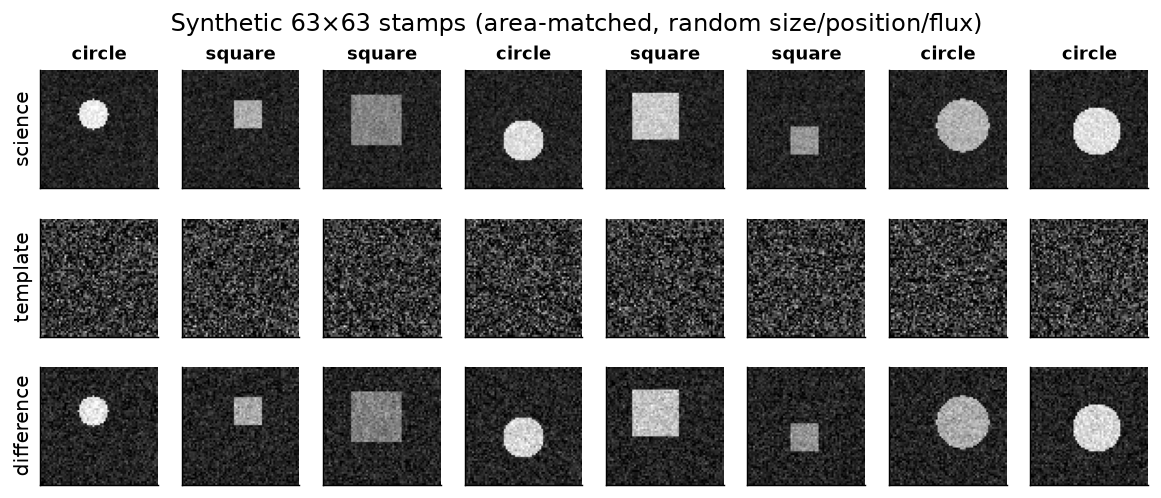
\includegraphics[width=\textwidth]{00_stamps.png}
  \end{columns}
\end{frame}

% ---------------------------------------------------------------------------
\begin{frame}{Yes: the latent separates circles from squares}
  \centering
  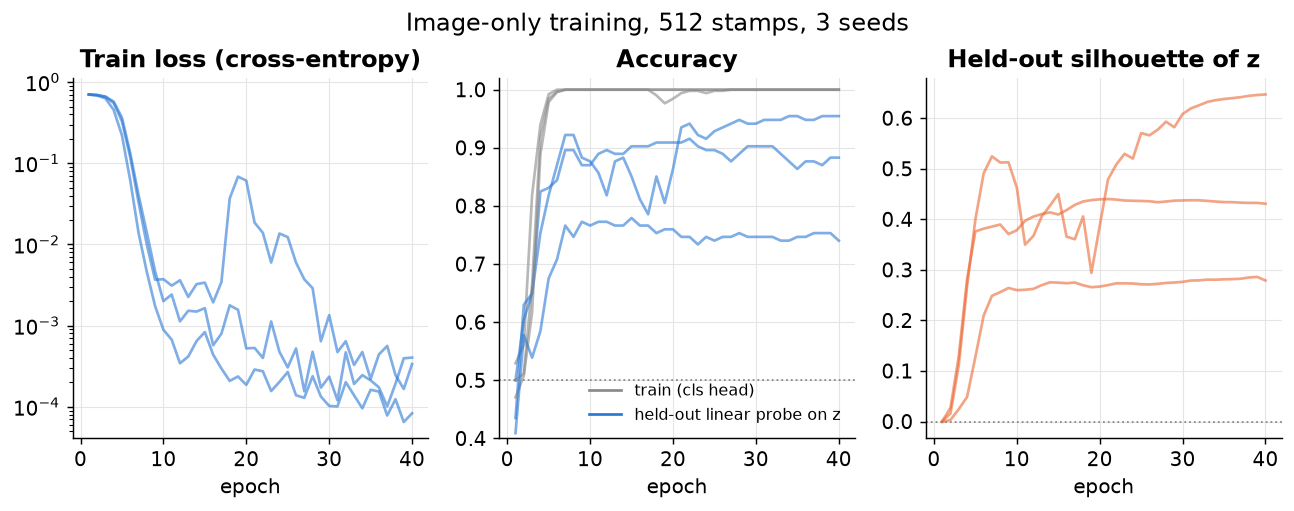
\includegraphics[width=0.82\textwidth]{01_training_curve.png}
  \begin{itemize}
    \item Training accuracy hits 100\,\% by epoch 6; held-out probe plateaus at 0.74--0.96
      depending on seed. Thus, the gap is generalization, not necessarily optimization.
    \item 512 stamps, simple 0.25\,M-parameter CNN, 30 epochs, $\sim$30\,s on CPU.
  \end{itemize}
\end{frame}

% ---------------------------------------------------------------------------
\begin{frame}{What the from-scratch CNN needs: data}
  \begin{columns}[T]
    \column{0.58\textwidth}
    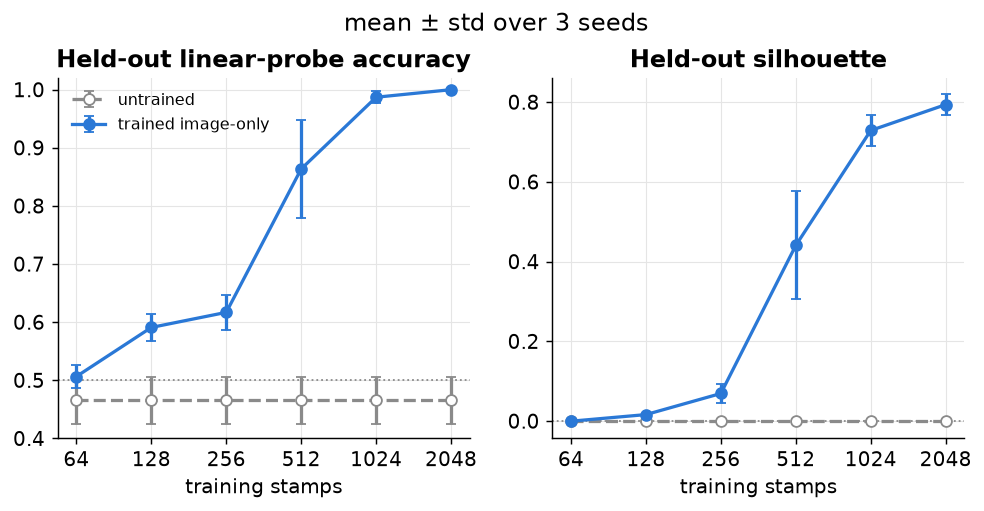
\includegraphics[width=\textwidth]{02_data_efficiency.png}
    \column{0.40\textwidth}
    \small
    \begin{tabular}{@{}rr@{}}
      \toprule
      training stamps & probe acc \\
      \midrule
      64   & 0.51 \\
      256  & 0.62 \\
      512  & 0.86 \\
      1024 & 0.99 \\
      2048 & 1.00 \\
      \bottomrule
    \end{tabular}
    \vspace{0.6em}

    Below $\sim$256 stamps nothing transferable is learned; the transition is
    between 256 and 1024.
  \end{columns}
\end{frame}

% ---------------------------------------------------------------------------
\begin{frame}{What the from-scratch CNN needs: signal, or more data}
  \begin{columns}[T]
    \column{0.58\textwidth}
    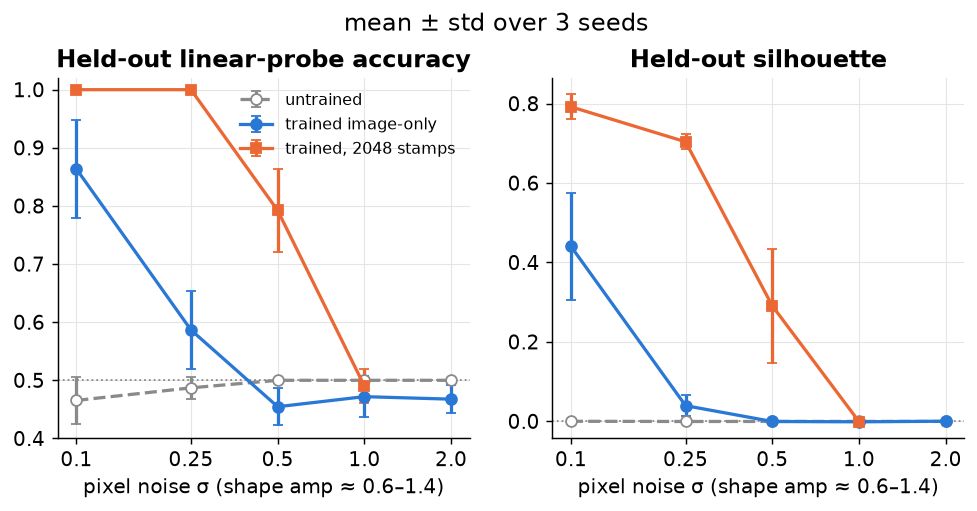
\includegraphics[width=\textwidth]{04_noise.png}
    \column{0.40\textwidth}
    \small
    \begin{tabular}{@{}rrr@{}}
      \toprule
      noise $\sigma$ & 512 st. & 2048 st. \\
      \midrule
      0.1  & 0.86 & 1.00 \\
      0.25 & 0.59 & 1.00 \\
      0.5  & 0.45 & 0.79 \\
      1.0  & 0.47 & 0.49 \\
      \bottomrule
    \end{tabular}
    \vspace{0.6em}

    Blob brightness is 0.6--1.4. At 512 stamps the model collapses to chance by
    $\sigma{=}0.5$; with 2048 it is fine at 0.25 and useful at 0.5.
    \alert{Thus, the main issue is data.}
  \end{columns}
\end{frame}

% ---------------------------------------------------------------------------
\begin{frame}{Things that do not matter: latent size, bottleneck type}
  \begin{columns}[T]
    \column{0.5\textwidth}
    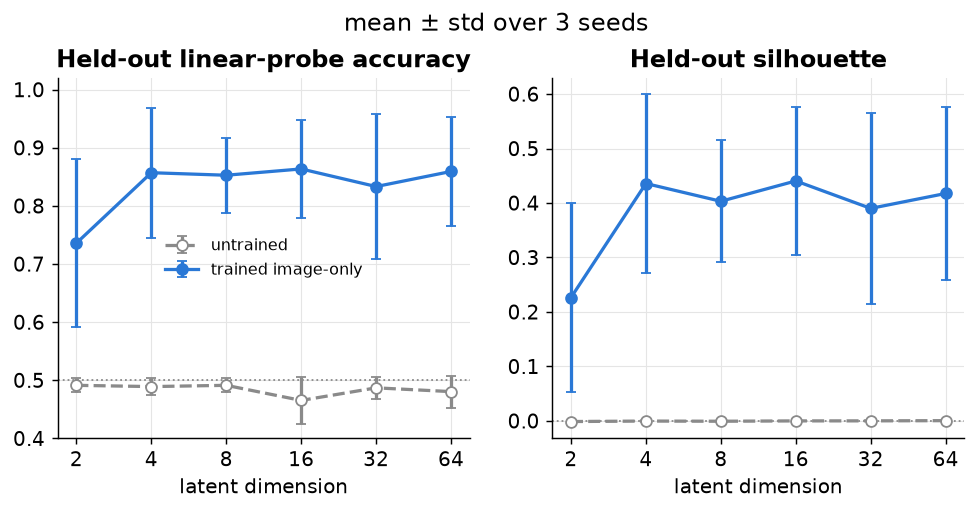
\includegraphics[width=\textwidth]{03_latent_dim.png}
    \column{0.5\textwidth}
    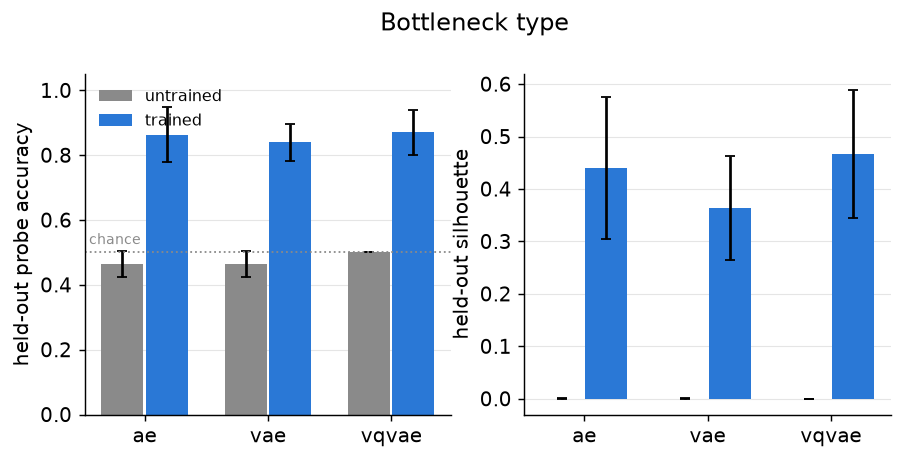
\includegraphics[width=\textwidth]{05_bottleneck_mode.png}
  \end{columns}
  \begin{itemize}
    \item Latent dim 4--64: all 0.83--0.86, within seed variance. 2-d works on 2 of 3 seeds.
    \item AE 0.86, VAE 0.84, VQ-VAE 0.87. Two classes do not stress the bottleneck.
  \end{itemize}
\end{frame}

% ---------------------------------------------------------------------------
\begin{frame}{The thing that matters: the pretrained backbone}
  \begin{columns}[T]
    \column{0.5\textwidth}
    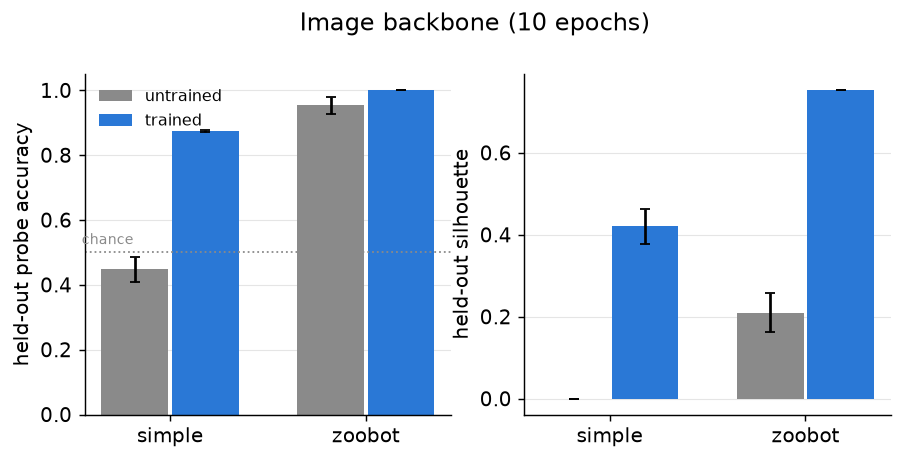
\includegraphics[width=\textwidth]{06_backbone.png}
    \column{0.5\textwidth}
    \small
    \begin{tabular}{@{}lrr@{}}
      \toprule
      backbone & probe before & after \\
      \midrule
      simple CNN (0.25\,M) & 0.45 & 0.87 \\
      Zoobot frozen (8.5\,M) & \textbf{0.93--0.98} & \textbf{1.00} \\
      \bottomrule
    \end{tabular}
    \vspace{0.6em}

    Galaxy Zoo features separate the shapes linearly through a \emph{random}
    projection, before any training. Training only the projection and bottleneck
    makes it perfect.
  \end{columns}
\end{frame}

% ---------------------------------------------------------------------------
\begin{frame}{Latent geometry: the class loss collapses $z$ to a line}
  \begin{columns}[T]
    \column{0.6\textwidth}
    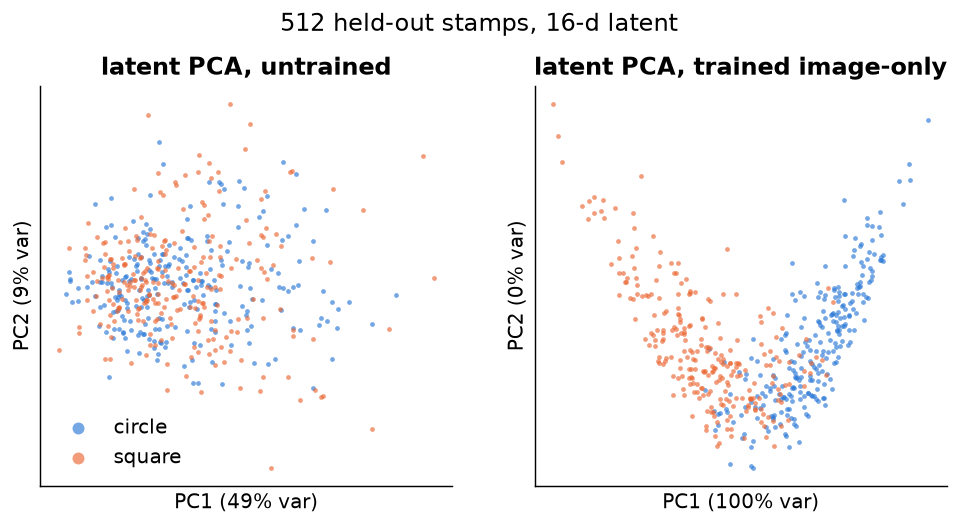
\includegraphics[width=\textwidth]{07_latent_pca.png}
    \column{0.38\textwidth}
    \begin{itemize}
      \item After classification-only training, PC1 explains 100\,\% of the variance.
      \item Expected here: there is nothing else to encode. But it is the mechanism
        behind the next part.
      \item In the real model the photometry reconstruction keeps the other
        dimensions alive; it does not protect \emph{image} information.
    \end{itemize}
  \end{columns}
\end{frame}

% ---------------------------------------------------------------------------
\begin{frame}{Part 2: can shapes the classifier never saw be found?}
  \begin{columns}[T]
    \column{0.5\textwidth}
    Train on circle/square only, then encode four unseen shapes:
    triangle, ring, ellipse, cross (area-matched, random orientation).
    \vspace{0.4em}

    \textbf{Read the latent without labels:}
    \begin{itemize}
      \item novelty: 5-NN distance to known-class latents (AUROC)
      \item clustering: $k$-means, $k{=}6$ (AMI)
      \item ceiling: 6-way probe \emph{with} labels
      \item geometry: participation ratio (16 = isotropic, 1 = line)
    \end{itemize}
    \column{0.5\textwidth}
    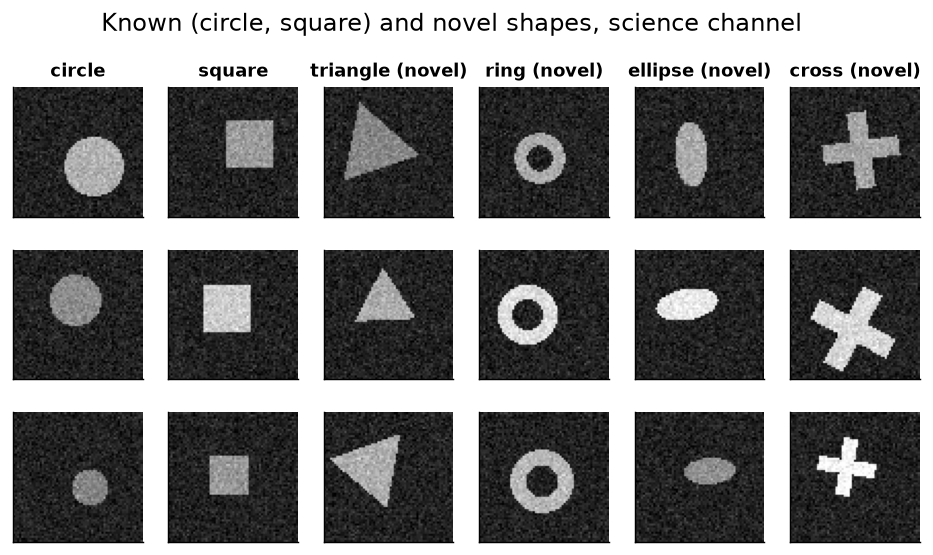
\includegraphics[width=\textwidth]{10_novel_stamps.png}
  \end{columns}
  \vspace{0.3em}
  \small Seven latents: untrained CNN; CNN with class loss, stamp reconstruction, or both;
  Zoobot frozen with no training; Zoobot frozen with class loss or both.
  \alert{Zoobot is never fine-tuned}; only projection, bottleneck and heads train.
\end{frame}

% ---------------------------------------------------------------------------
\begin{frame}{Results across the seven latents}
  \centering
  \small
  \begin{tabular}{@{}lcccc@{}}
    \toprule
    latent regime & probe (labels) & novelty AUROC & $k$-means AMI & eff.\ dims \\
    \midrule
    untrained CNN            & 0.23 & 0.55 & 0.00 & 3.3 \\
    CNN, class loss          & 0.43 & 0.68 & 0.28 & \textbf{1.0} \\
    CNN, reconstruction      & 0.34 & 0.75 & 0.01 & 5.2 \\
    CNN, both                & 0.44 & 0.68 & 0.23 & 2.7 \\
    Zoobot frozen, untrained & \textbf{0.995} & \textbf{0.998} & 0.54 & 4.8 \\
    Zoobot, class loss       & 0.85 & 0.96 & 0.54 & \textbf{1.0} \\
    Zoobot, both             & 0.97 & 0.97 & \textbf{0.62} & 1.4 \\
    \bottomrule
  \end{tabular}
  \vspace{0.6em}

  \begin{itemize}
    \item No from-scratch CNN latent finds the novel shapes, whatever the loss.
    \item The frozen Zoobot latent finds all four with \emph{zero} training.
    \item The class loss flattens every latent to one effective dimension, Zoobot included.
  \end{itemize}
\end{frame}

% ---------------------------------------------------------------------------
\begin{frame}{What the latents look like}
  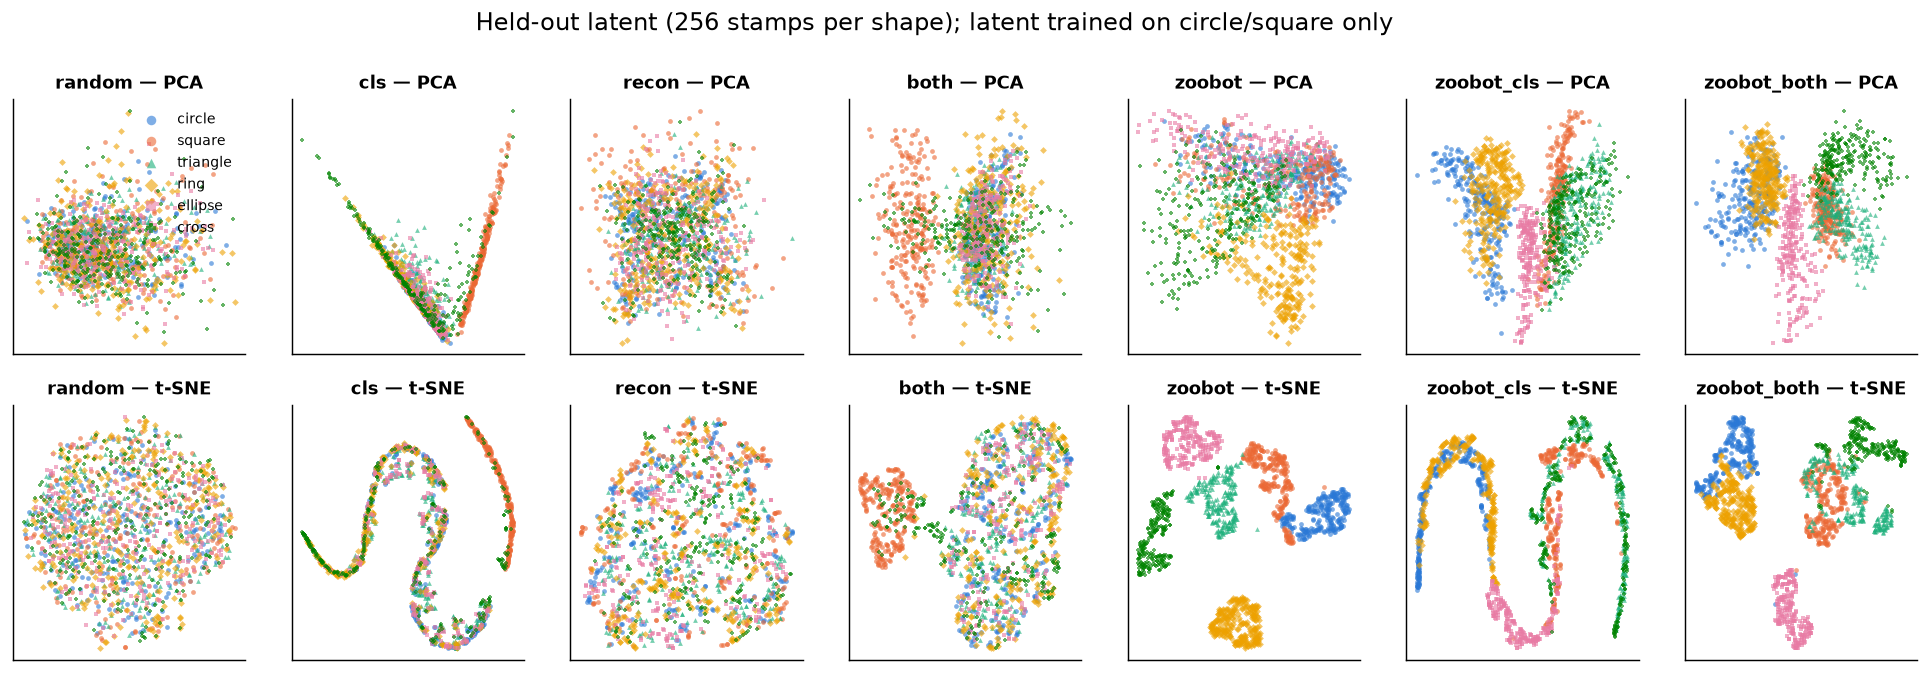
\includegraphics[width=\textwidth]{11_novel_latent_views.png}
  \footnotesize Top: PCA (honest linear view). Bottom: t-SNE (exaggerates separation).
  Class-trained CNN: a V with novel shapes along the circle--square axis.
  Zoobot untrained: ring and cross clearly apart; triangle and ellipse overlap in PCA.
\end{frame}

% ---------------------------------------------------------------------------
\begin{frame}{Label-free novelty and clustering}
  \begin{columns}[T]
    \column{0.56\textwidth}
    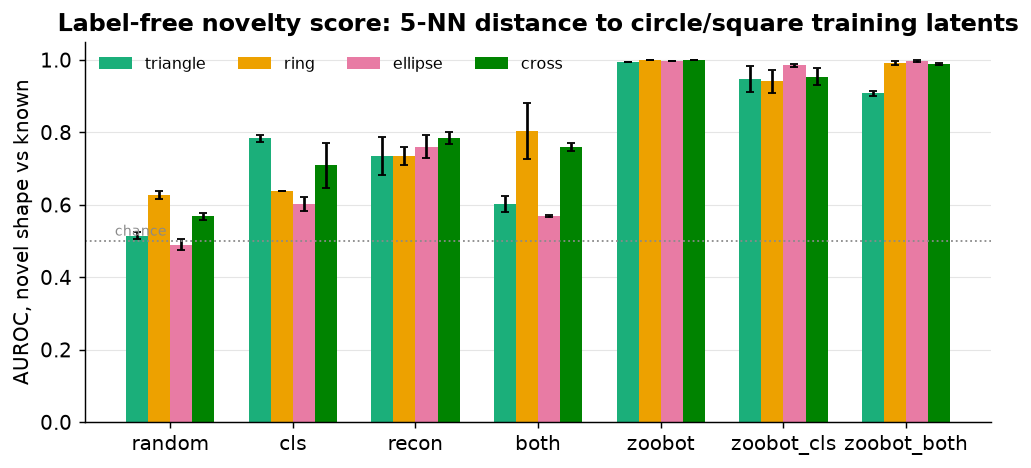
\includegraphics[width=\textwidth]{12_novelty_auroc.png}
    \column{0.42\textwidth}
    \small
    \begin{itemize}
      \item Class-trained CNN calls 100\,\% of triangles, rings and ellipses
        ``circle'' with full confidence: classifier confidence is at chance as a
        novelty signal.
      \item Zoobot untrained: ring gets a pure cluster (95\,\% recall, 100\,\%
        purity); triangle and ellipse share one, which caps the AMI at 0.54.
      \item Zoobot with class loss: 1-d latent, probe drops 0.995\,$\to$\,0.85,
        but each novel shape still owns its own stretch of the curve (AUROC 0.96).
    \end{itemize}
  \end{columns}
\end{frame}

% ---------------------------------------------------------------------------
\begin{frame}{What this does and does not prove}
  \textbf{Does prove}
  \begin{itemize}
    \item Pretrained Zoobot features retain information about classes never trained on;
      a CNN trained from scratch on two classes learns a two-class detector and nothing else.
    \item Discoverability lives in the backbone, not in the transformer, bottleneck or head.
    \item The joint classification loss is the main threat to it.
  \end{itemize}
  \textbf{Does not prove (yet)}
  \begin{itemize}
    \item That \emph{Galaxy Zoo} pretraining specifically is the reason. Missing controls:
      ImageNet-pretrained ConvNeXt-pico and a random-init ConvNeXt-pico, both cheap.
    \item Anything about real stamps: hosts, PSF, faint transients. The toy flatters any
      pretrained encoder.
    \item That Zoobot is better at the \emph{trained} task; with 2048 stamps the CNN also
      reached 1.00.
  \end{itemize}
\end{frame}

% ---------------------------------------------------------------------------
\begin{frame}{Takeaways and next steps}
  \begin{itemize}
    \item The cutout pathway works and the latent is image-informative.
    \item From-scratch image tower: needs $\gtrsim$1000 stamps and clean signal, and discards
      everything but the trained classes.
    \item Frozen Zoobot: data-efficient, noise-tolerant on this toy, and keeps unseen
      structure findable without labels.
    \item Next: run the ImageNet and random-init ConvNeXt controls; then measure the
      class-loss collapse on real alerts with \texttt{eval\_discovery.py}.
  \end{itemize}
  \vspace{0.5em}
  \footnotesize Code: \texttt{src/sanity\_shapes.py}, \texttt{src/shape\_experiments.py},
  \texttt{src/shape\_novelty.py}. Write-up with all figures and raw JSON:
  \texttt{docs/shape\_baseline.md}. Tests: \texttt{tests/test\_shapes.py},
  \texttt{tests/test\_novelty.py}.
\end{frame}

\end{document}
